\documentclass{beamer}

\usepackage[utf8]{inputenc}
\usepackage[T1]{fontenc}
\usepackage{tikz}
\usepackage{fontspec}
\usepackage{wrapfig}
\usepackage{float}
\usepackage{amsmath}
\usepackage{varwidth}
\usepackage[font=scriptsize]{caption}
\usepackage{graphicx}

\usetheme{metropolis}
\usetikzlibrary{matrix}
\usetikzlibrary{calc}
\usetikzlibrary{external}
\setmainfont[Ligatures=TeX]{Fira Sans}

\title{Don Quixote}

\date{\vspace{1em}Zagreb, 21. siječnja 2020.}

\institute{Fakultet elektrotehnike i računarstva}

\author{Marko Lazarić (voditelj)  \\ Matija Bačić \hspace*{10em} Bruno Bandić \\ Darijo Brčina \hspace*{9.75em} Jakov Ćurić \\ Andrija Raguž \hspace*{9.3em} Nikola Vnučec \\[1em] Mentor: Doc. dr. sc. Marko Čupić}

\newcommand{\engl}[1]{ (engl. \emph{#1})}
\newcommand{\twocolumns}[2]{
	\begin{columns}
		\begin{column}{0.4\textwidth}
			#1
		\end{column}
		\begin{column}{0.6\textwidth}  %%<--- here
			#2
		\end{column}
	\end{columns}
}
%\setbeameroption{show notes}
%\setbeamertemplate{note page}[plain]
\renewcommand{\figurename}{Slika}

\begin{document}
  \begin{frame}[noframenumbering, plain]
  	\centering
  	\vspace{2em}
  	Preddiplomski projekt
  	\vspace{-4em}
  	
  	\titlepage
  \end{frame}

  \begin{frame}{Komponente}
	\tableofcontents
  \end{frame}

  \section{Igra Don Quixote}
      
  \begin{frame}{Inspiracija}
  	\vspace{3em}
  	\twocolumns {
  		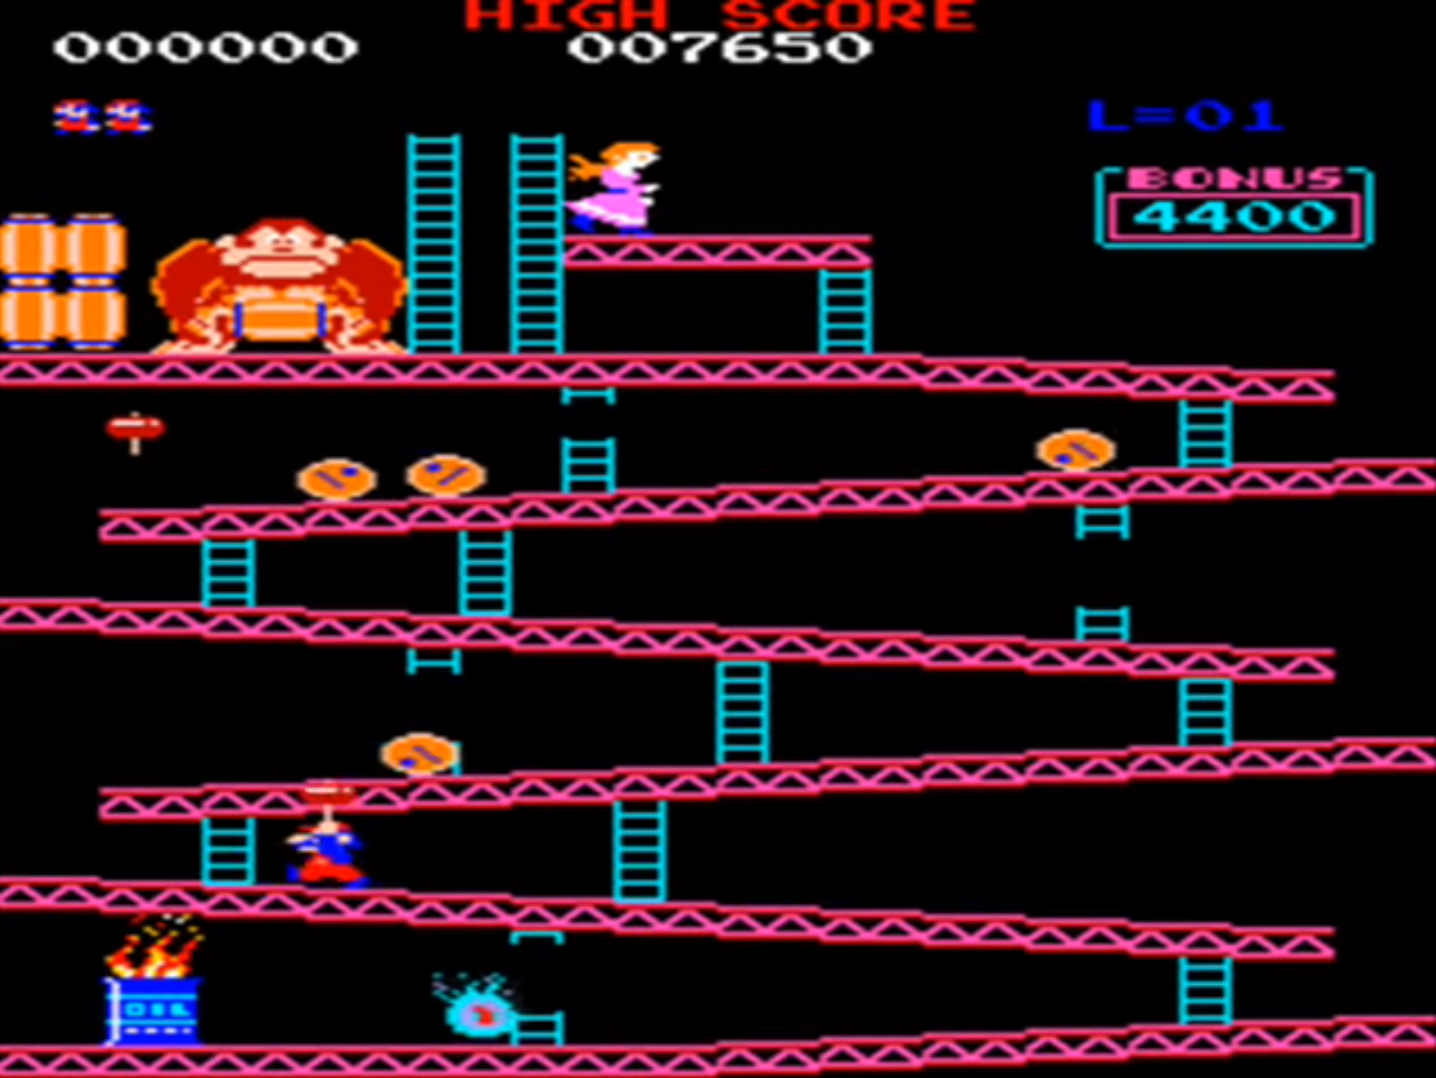
\includegraphics[width=1.2\textwidth]{slike/donkeykong_game}
  	} {
  	  \vspace{1em}
	  \hspace{3em}\fbox{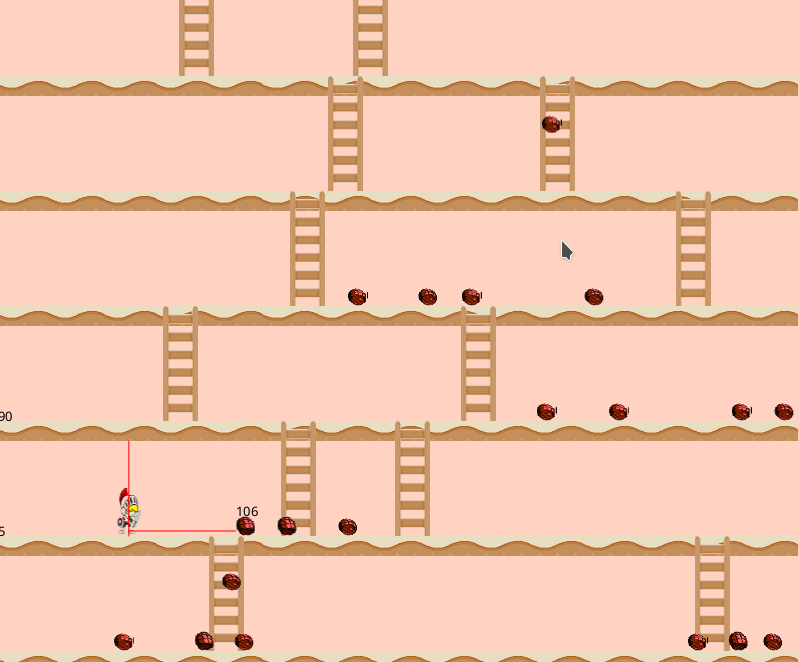
\includegraphics[width=0.7\textwidth]{slike/donquixote_game}}
  	}
  \end{frame}

	\begin{frame}{Inspiracija}
		\hspace{4em}\fbox{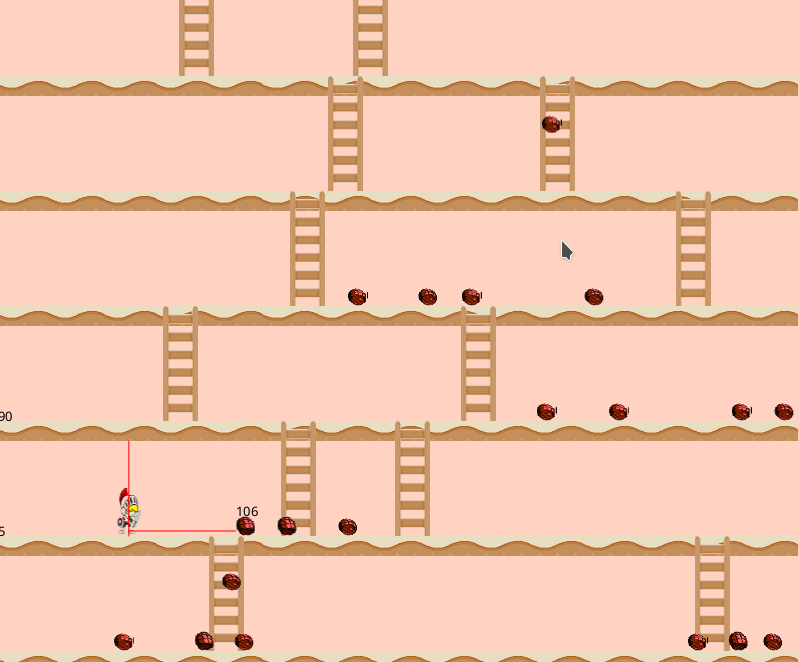
\includegraphics[width=0.7\textwidth]{slike/donquixote_game}}
	\end{frame}

  \begin{frame}{Pokretački sklop (eng. \textit{Game engine})}
  	\begin{itemize}
  		\item Diskretni otkucaji sata (eng. \textit{ticks})
  		\item Stroj stanja (eng. \textit{State machine}), oblikovni obrazac promatrač
  		\item 4 koraka:
  		\begin{enumerate}
  			\item Izračun pomaka igrača i svih ostalih objekata
  			\item Korekcija pomaka
  			\item Izračun kolizija svih objekata međusobno (uključujući i igrača)
  			\item Izračun novih brzina svih objekata 
  		\end{enumerate}
  	\end{itemize}
  	\hspace{5em}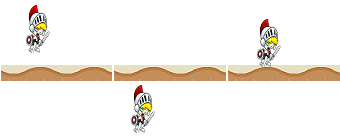
\includegraphics[width=0.65\textwidth]{slike/positionCorrection}
  \end{frame}

  \begin{frame}{Pravila igre i potezi}
  \end{frame}

  \begin{frame}{Ulazni podaci umjetnom igraču na temelju sudara zraka}
  \end{frame}


  \section{Modeli umjetne inteligencije}
  \begin{frame}{Unaprijedna umjetna neuronska mreža}
	\twocolumns{
\begin{figure}
	
	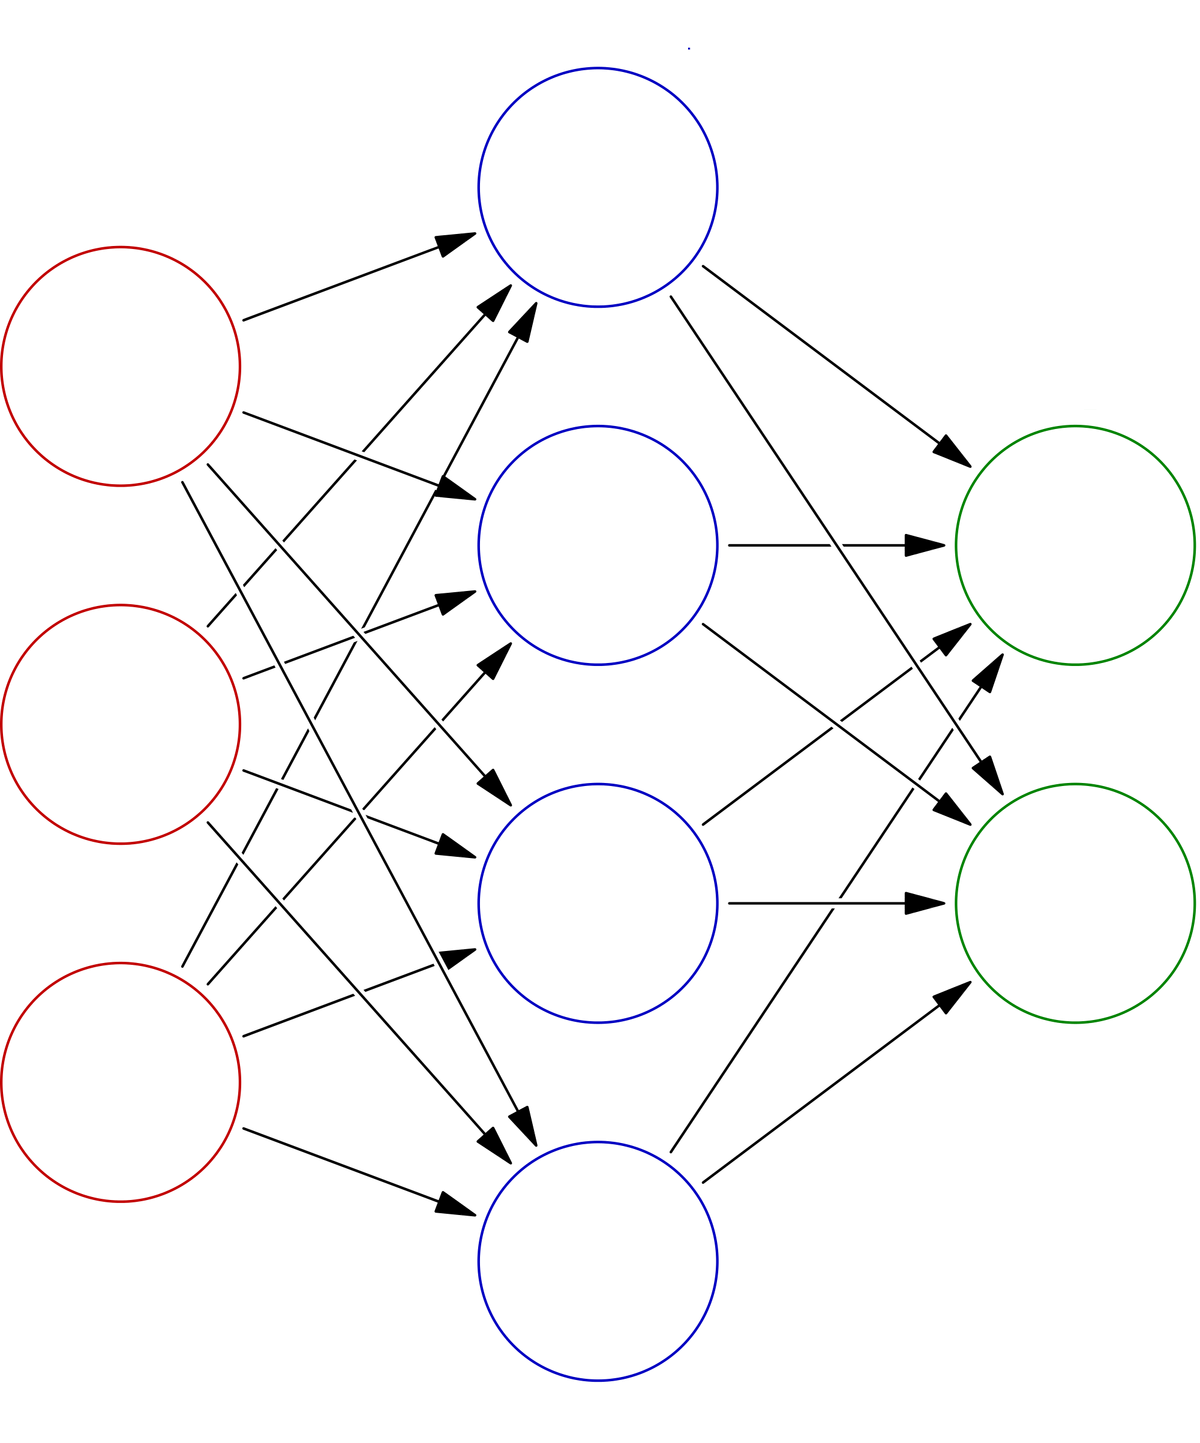
\includegraphics[width=1\textwidth]{slike/unaprijedna}
	\caption{Unaprijedna umjetna neuronska mreža \\ Izvor: automaticaddison, \textit{Artificial Feedforward Neural Network With Backpropagation From Scratch}}
\end{figure}
	}{
		\begin{itemize}
			\item \textbf{ulaz:} polje realnih brojeva iz igre dovodimo na ulazni sloj
			\item \textbf{izlaz:} igrač je odigrao akciju s najvećom vrijednosti u izlaznom sloju
			\item \textbf{u memoriji:} polje realnih brojeva (težine)
		\end{itemize}
	}
\end{frame}

\begin{frame}{Elmanova umjetna neuronska mreža}
	\twocolumns{
	\begin{figure}
	
	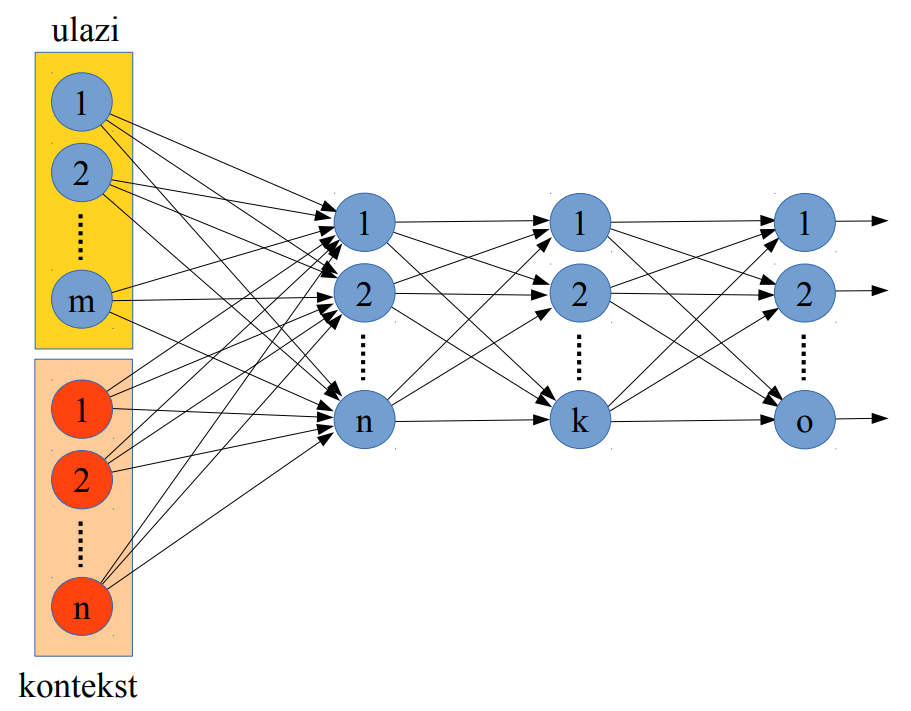
\includegraphics[width=1.25\textwidth]{slike/elman}
	\caption{Elmanova umjetna neuronska mreža \\ Izvor: Čupić, M. \textit{8. domaća zadaća – algoritam diferencijske evolucije}}
\end{figure}
}{
		\begin{itemize}
			\item \textbf{ulaz:} polje realnih brojeva iz igre dovodimo na ulazni sloj
			\item \textbf{izlaz:} igrač je odigrao akciju s najvećom vrijednosti u izlaznom sloju
			\item \textbf{u memoriji:} polje realnih brojeva (početne vrijednosti kontekstnog sloja i težine)
		\end{itemize}
	}
\end{frame}

\begin{frame}{Operatorsko stablo}
	\twocolumns{
\begin{figure}
\begin{forest}
for tree={
  l sep=30pt,
  parent anchor=south,
  align=center
}
[+
  [*,edge label={node[midway,left]{}}
    [-,edge label={node[midway,left]{}}
      [{[4]},edge label={node[midway,left]{}}
      ]
      [{[5]},edge label={node[midway,right]{}}
      ]
    ]
    [{[3]},edge label={node[midway,right]{}}
    ]
  ]
  [/,edge label={node[midway,right]{}}
	[{[3]},edge label={node[midway,left]{}}
    ]
    [{[5]},edge label={node[midway,right]{}}
    ]
  ]
]
\end{forest}
\caption{Operatorsko stablo za funkciju $([4] - [5]) \cdot [3] + [3] / [5]$}
\end{figure}
}{
		\begin{itemize}
			\item \textbf{ulaz:} polje realnih brojeva iz igre dovodimo na ulaz
			\item \textbf{izlaz:} igrač je odigrao akciju s indeksom $\floor{6 \cdot \frac{\sin{x} + 1}{2}}$
			\item \textbf{u memoriji:} stablo
		\end{itemize}
	}
\end{frame}

\begin{frame}{Programski isječak}
	\twocolumns{
\begin{figure}
\verbatiminput{test.lgp}
\caption{LGP program za izračun $R8 = (R4 - R5) \cdot R3 + R3 / R5$}
\end{figure}
}{
		\begin{itemize}
			\item \textbf{ulaz:} polje realnih brojeva iz igre ugradimo u registre
			\item \textbf{izlaz:} igrač je odigrao akciju s indeksom $\floor{6 \cdot \frac{\sin{\mathrm{R0}} + 1}{2}}$
			\item \textbf{u memoriji:} lista instrukcija
		\end{itemize}
	}
\end{frame}


  \section{Optimizacijski algoritmi}
  \begin{frame}{Genetski algoritam}
	\begin{itemize}
		\item generacijski genetski algoritam
		\item operatori:
		\begin{itemize}
			\item $k$-turnirska selekcija
			\item BLX-$\alpha$ križanje
			\item normalna mutacija
		\end{itemize}
		\item modeli:
		\begin{itemize}
			\item unaprijedna umjetna neuronska mreža
			\item Elmanova umjetna neuronska mreža
		\end{itemize}
	\end{itemize}
\end{frame}

\begin{frame}{Diferencijska evolucija}
	\begin{itemize}
		\item strategije:
		\begin{itemize}
			\item DE/rand/1/bin
			\item DE/target-to-best/4/bin
		\end{itemize}
		\item modeli:
		\begin{itemize}
			\item unaprijedna umjetna neuronska mreža
			\item Elmanova umjetna neuronska mreža
		\end{itemize}
	\end{itemize}
\end{frame}

\begin{frame}{Genetsko programiranje bazirano na operatorskim stablima}
	\begin{itemize}
		\item generacijski genetski algoritam s elitizmom
		\item operatori:
		\begin{itemize}
			\item $k$-turnirska selekcija
			\item zamjena podstabla jednog roditelja podstablom drugog roditelja 
			\item zamjena podstabla slučajno generiranim podstablom
		\end{itemize}
		\item modeli:
		\begin{itemize}
			\item operatorsko stablo
		\end{itemize}
	\end{itemize}
\end{frame}

\begin{frame}{Linearno genetsko programiranje}
	\begin{itemize}
		\item generacijski genetski algoritam
		\item operatori:
		\begin{itemize}
			\item proporcionalna selekcija
			\item križanja:
			\begin{itemize}
				\item križanje s jednom točkom prekida
				\item križanje s dvije točke prekida
			\end{itemize}
			\item mutacije:
			\begin{itemize}
				\item zamjena jedne instrukcije slučajno generiranom instrukcijom
				\item zamjena kontinuiranog bloka instrukcija slučajno generiranim blokom instrukcija
			\end{itemize}
		\end{itemize}
		\item modeli:
		\begin{itemize}
			\item programski isječak
		\end{itemize}
	\end{itemize}
\end{frame}


  \section*{Demonstracija programa}

  \begin{frame}{Diskusija: male scene}
  \end{frame}

  \begin{frame}{Diskusija: generalizirano ponašanje}
  \end{frame}
  
  \begin{frame}[plain]
  	\section*{Hvala na pažnji!}
  	\usebeamerfont{frametitle}
  	\hspace{15em}Pitanja?
  \end{frame}
  
\end{document}